Fram að þessu höfum við skoðað aðferðir sem finna bestu lausn á há- eða lágmörkunarverkefnum sbr. Simplex-aðferðin fyrir línulega bestun og \emph{branch and bound} fyrir heiltölubestun.

Mörg hagnýt verkefni í aðgerðagreiningu eru af þeirri stærðargráðu að illmögulegt eða jafnvel ómögulegt er að finna bestu lausn.

Í slíkum tilfellum er ásættanlegt að finna \emph{góða} lausn, þ.e. gjaldgenga lausn sem er ekki mikið verri en sú besta.

Svonefndar \ath{brjóstvitsaðferðir} (e. heuristics) eru oft notaðar til að finna slíkar nálgunarlausnir.

Eitt þekktasta dæmið snýst um farandsölumann (e. Travelling Salesman Problem -- TSP) sem ætlar að heimsækja nokkra bæi. Verkefnið felst í því að heimsækja sérhvern bæ einu sinni áður en hann snýr til baka í bæinn sem hann býr í, þannig að heildarvegalengd sé sem minnst.

\begin{daemi}[TSP]\label{daemi:tsp}\hspace{.1cm}
\begin{center}
  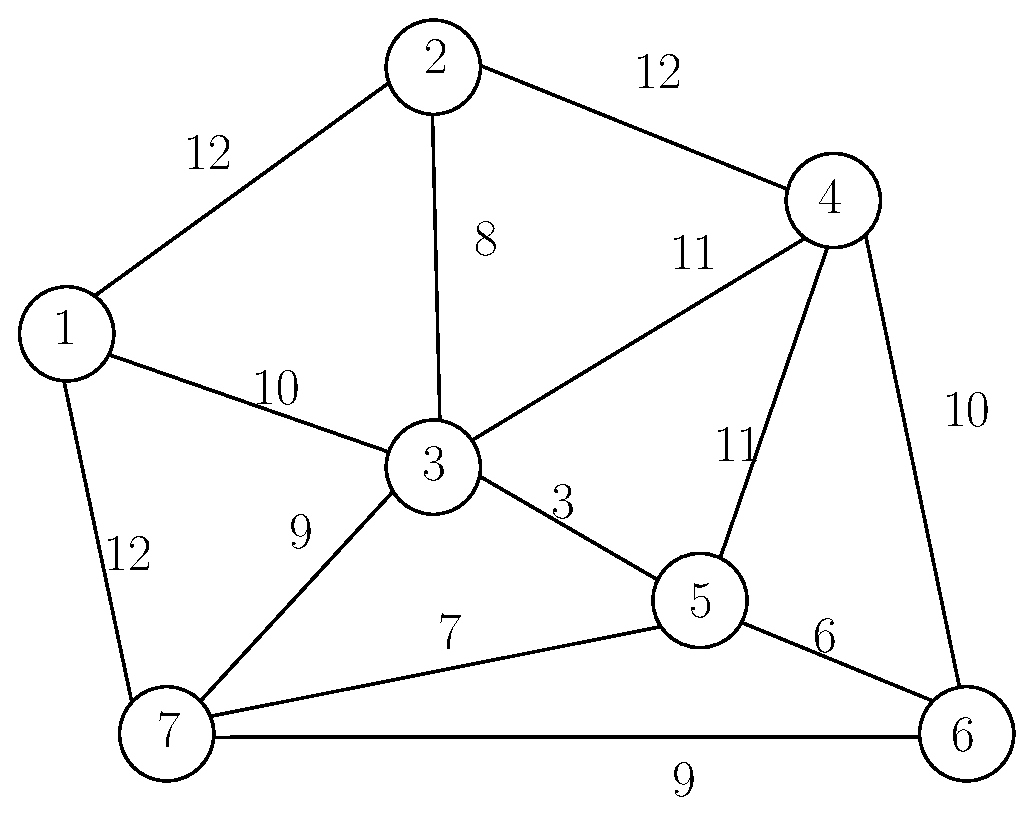
\includegraphics[width=0.6\columnwidth]{figs/tsp.eps}
\end{center}
\end{daemi}

Skyld verkefni eru m.a.
\begin{itemize}
  \item Vöruútkeyrsla
  \item Framleiðsla á prentplötum
\end{itemize}

\begin{aths}Fjöldi mögulegra leiða ef fjöldi bæja er $n$ er:
$$ \frac{(n-1)(n-2)\cdots(1)}{2}=\frac{(n-1)!}{2}$$
Þannig að fyrir $n=20$ eru þetta $10^{16}$ gjaldgengar leiðir, en fyrir $n=50$ eru þetta $10^{62}$ gjaldgengar leiðir!  
\end{aths}

Framgangsmáti nálgunaraðferða er yfirleitt þannig að fyrst er fundin einhver gjaldgeng lausn (getur verið mjög erfitt) og síðan eru smávægilegar bætingar á lausninni gerðar ítrekað.

Dæmi um slíkar endurbætur í verkefni farandsölumannsins er að víxla á tveimur eða fleiri áfangastöðum (e. subtour reversal).

\begin{lausnSYND}[á TSP dæmi \ref{daemi:tsp}]Höfum gefna upphafslausn þar sem farandsölumaðurinn fer $1\to2\to3\to4\to5\to6\to7\to1$ með fjarlægð 69.
\begin{center}
  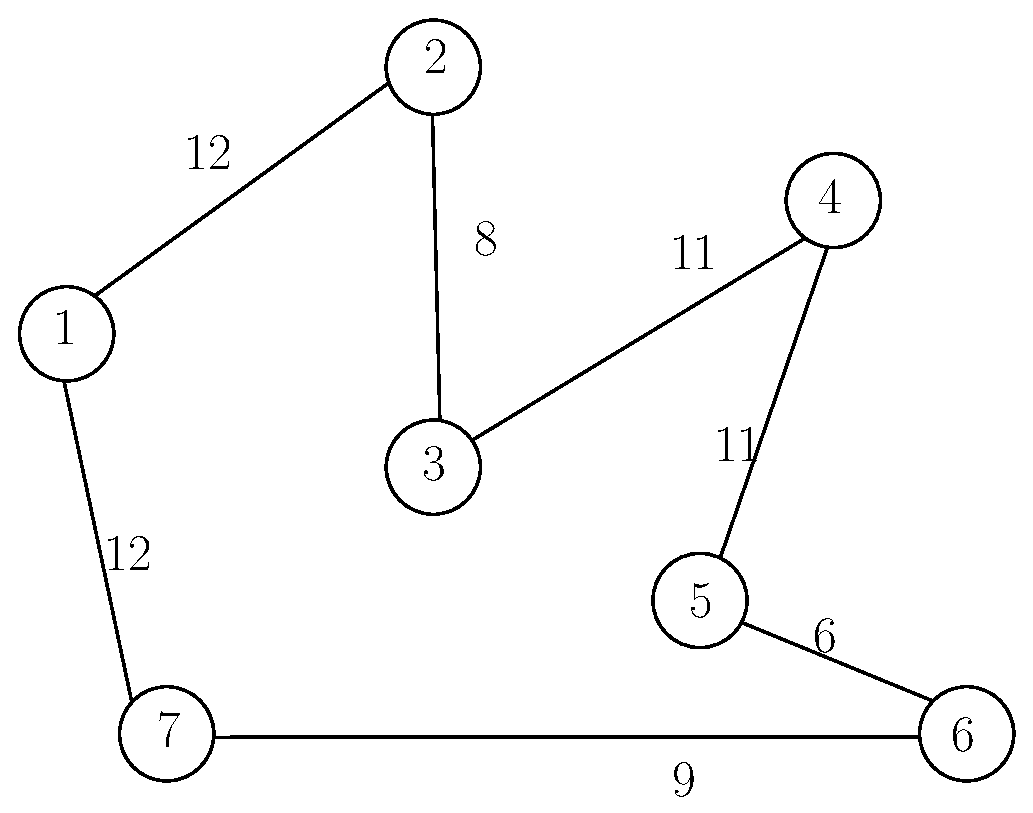
\includegraphics[width=0.6\columnwidth]{figs/tsp_12345671.eps}
\end{center}
Prófum að víxla á $2\to3,3\to4,4\to5$ og $5\to6$. 
\newpage
Ef víxlað er t.d. á $3\to4$ verður vegalengdin 65 -- sem er stytting um 4.
\begin{center}
  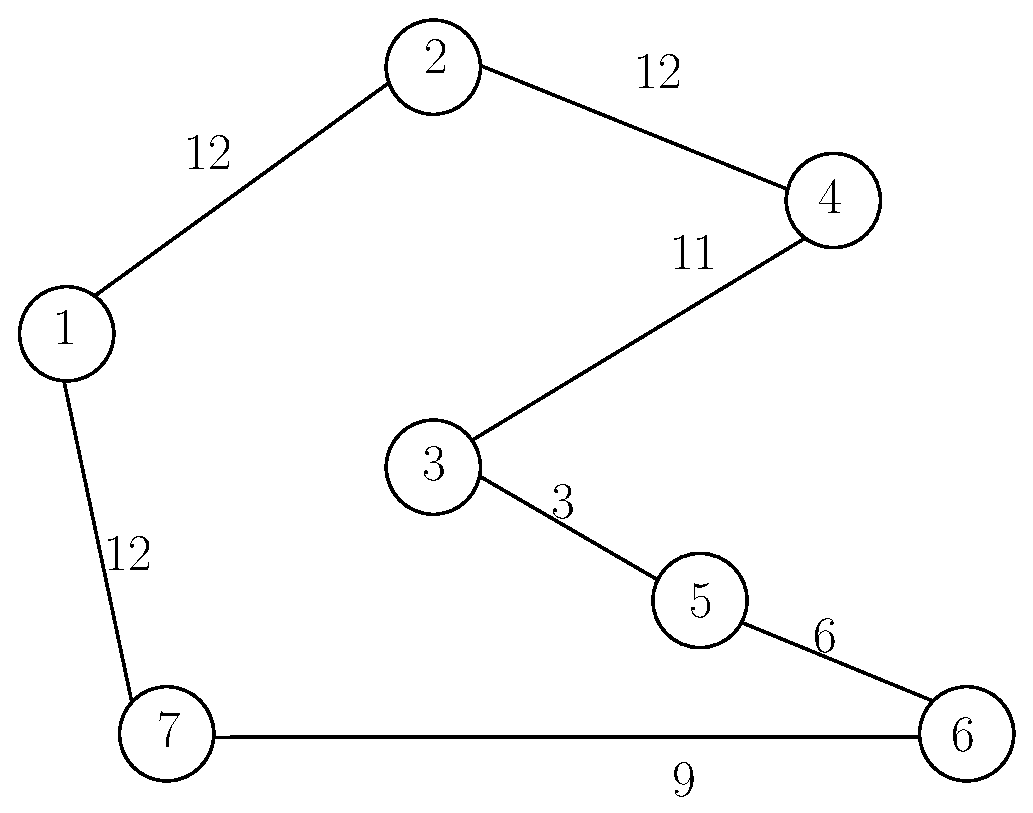
\includegraphics[width=0.5\columnwidth]{figs/tsp_12435671.eps}
\end{center}

Á sama  hátt fæst
\begin{center}
  \begin{tabular}{|c|c|c|ll}\cline{1-3}
    Víxlað & Leið & Vegalengd \\ \cline{1-3}
        & $1-2-3-4-5-6-7-1$ & 69 \\
$2\to3$ & $1-3-2-4-5-6-7-1$ & 68 \\
$3\to4$ & $1-2-4-3-5-6-7-1$ & \fbox{65} & $\nwarrow$\multirow{2}{*}{Mesta bæting}\\
$4\to5$ & $1-2-3-5-4-6-7-1$ & \fbox{65} & $\swarrow$\\
$5\to6$ & $1-2-3-4-6-5-7-1$ & 66 \\ \cline{1-3}
  \end{tabular}
\end{center}
Veljum t.d. $1-2-4-3-5-6-7-1$ (sjá mynd hér að ofan). Hægt er að stytta enn frekar m.þ.a. víxla $3-5-6$, og fá vegalend 64.
\begin{center}
  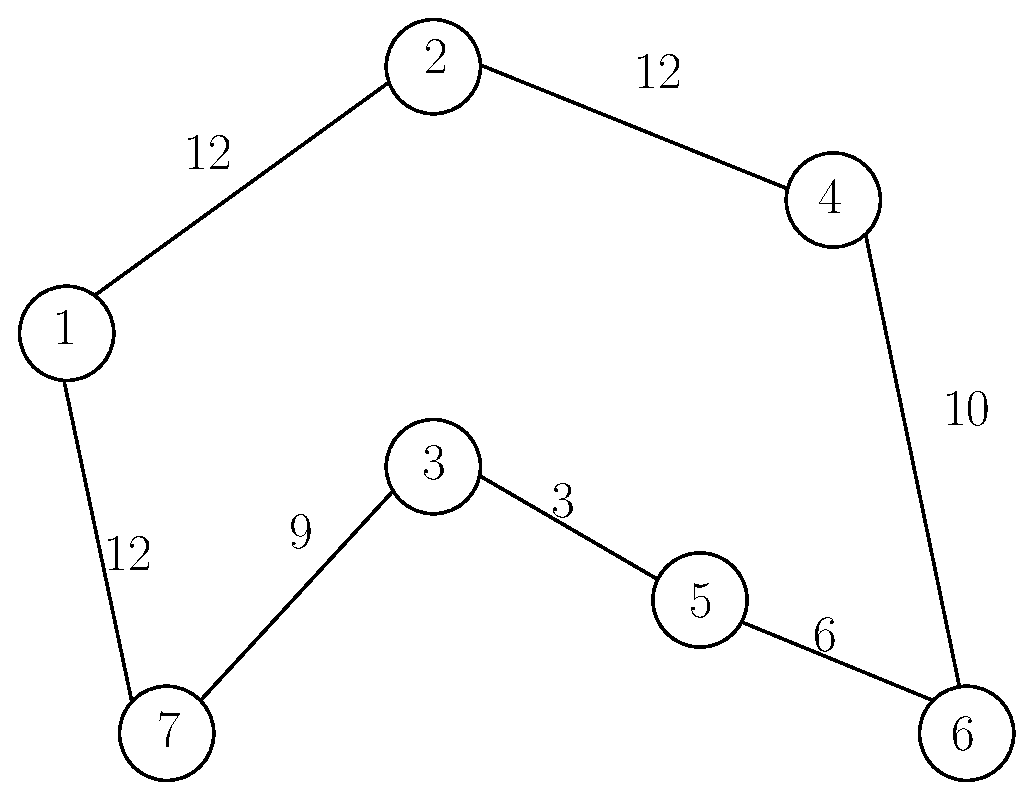
\includegraphics[width=0.5\columnwidth]{figs/tsp_12465371.eps}
\end{center}
Ekki er hægt að stytta vegalend meira með þessari aðferð. Hún finnur því \emph{ekki} bestu lausn, $1-2-4-6-7-5-3-1$  með vegalengd 63.

Við segjum að aðferðin sé föst í \emph{staðbundnu lággildi} (e. local optimum).

  
\end{lausnSYND}

\begin{samepage}
\begin{lausn}[Heiltöluframsetning á TSP \ref{daemi:tsp}]
Gefið:
\begin{enumerate}
  \item[$\mathcal{V}$] mengi hnúta,
  \item[$\mathcal{E}$] mengi leggja $\mathcal{E}\subset \mathcal{V}\times\mathcal{V}$,
  \item[$c_{ij}$] vegalengd frá $i$ til $j$,
  \item[$n$] fjöldi hnúta, $n=|\mathcal{V}|$.
\end{enumerate}
Ákvarðanabreytur:
\[ x_{ij}=\Bigg\{\begin{array}{cl}1 & \textrm{ef sölumaður fer úr bæ $i$ til bæ $j$} \\ 0 & \textrm{annars}\end{array}\]
Markfall 
\[ \min_{\vec{x}} \sum_{(i,j)\in\mathcal{E}}c_{ij}x_{ij}\]
m.t.t. skorða
\begin{eqnarray*}
  \sum_{j:\;(i,j)\in\mathcal{E}}x_{ij}=1 &\quad \forall i\in\mathcal{V}\quad & \mbox{yfirgefur bæ $i$ einu sinni}\\
  \sum_{i:\;(i,j)\in\mathcal{E}}x_{ij}=1 &\quad \forall j\in\mathcal{V}\quad & \mbox{förum einu sinni í bæ }j\\
\end{eqnarray*}

  \begin{aths}
    Þessar skorður duga ekki til -- því við getum fengið ósamanhangandi lausnir.
  \end{aths}

Margar leiðir eru þekktar t.þ.a. tryggja það að lokalausn sé samanhangandi. Ein slík er að láta sölumanninn selja nákvæmlega einn hlut í hverjum bæ. Bætum við ákvarðanabreytu:
\begin{enumerate}
  \item[$y_{ij}$] Fjöldi hluta sem sölumaður á eftir að hafa yfirgefið bæ $i$ og áður en hann kemur í bæ $j$ (flæði um legg $(i,j)$), $y_{ij}\geq0$. 
\end{enumerate}
og skorðum
\[y_{ij} \leq (n-1)x_{ij} \quad\quad\forall(i,j)\in\mathcal{E} \]
\begin{eqnarray*}
  \sum_{j:\;(j,i)\in\mathcal{E}}y_{ji}&=&\sum_{j:\;(i,j)\in\mathcal{E}}y_{ij}+1\quad\forall i\in\mathcal{V}\backslash\{i\} \\
  \sum_{j:\;(j,i)\in\mathcal{E}}y_{ji}+n&=&\sum_{j:\;(i,j)\in\mathcal{E}}y_{ij}+1\quad i=1 
\end{eqnarray*}
\begin{aths}Getum notað \textsc{glpk} t.þ.a. leysa TSP með 16--20 bæjum.\end{aths}
\end{lausn}
\end{samepage}

Bestunarverkefni sem hafa fleiri en eitt \ath{staðbundið lággildi} (e. local optimum) eru sögð vera \ath{víðvær} (e. global).


\begin{daemi}
  Hámarka $f(x)=12x^5-975x^4+28000x^3-345000x^2+1800000x$ með $0\leq x\leq 31$. 
\end{daemi}
\begin{lausnSYND}
Rissum upp feril fallsins og finnum þannig hágildispunktinn.
\begin{center}
  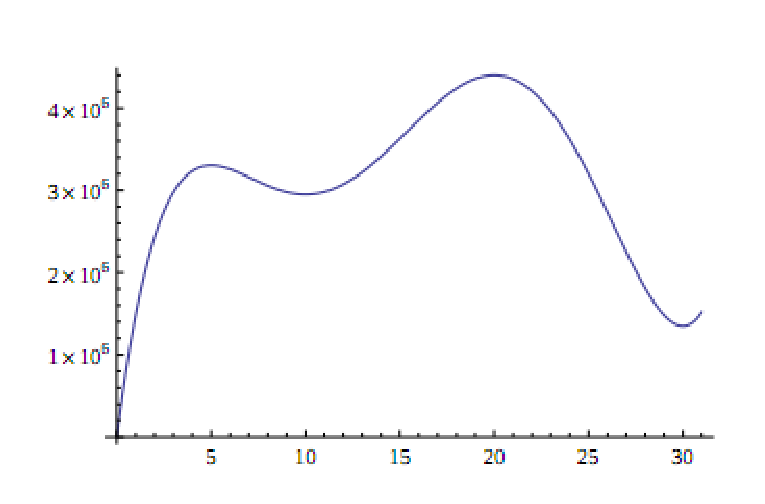
\includegraphics[width=0.5\columnwidth]{figs/global_opt.eps}
\end{center}
\end{lausnSYND}


\begin{daemi}
  Hámarka $f(x)=\cos(x_1)^2+\sin(x_2)^2$ með $-5\leq x_1\leq 5$, $-5\leq x_2\leq 5$. 
\end{daemi}
\begin{lausnSYND}
  Rissum feril fallsins með \textsc{Matlab} á eftirfarandi hátt:
\begin{lstlisting}[language=matlab]
>> [x1,x2]=meshgrid(-5:0.1:5,-5:0.1:5);
>> f=cos(x1).^2+sin(x2).^2;
>> surf(x1,x2,f);
>> shading interp
>> xlabel('x1'), ylabel('x2')
\end{lstlisting}
\begin{center}
  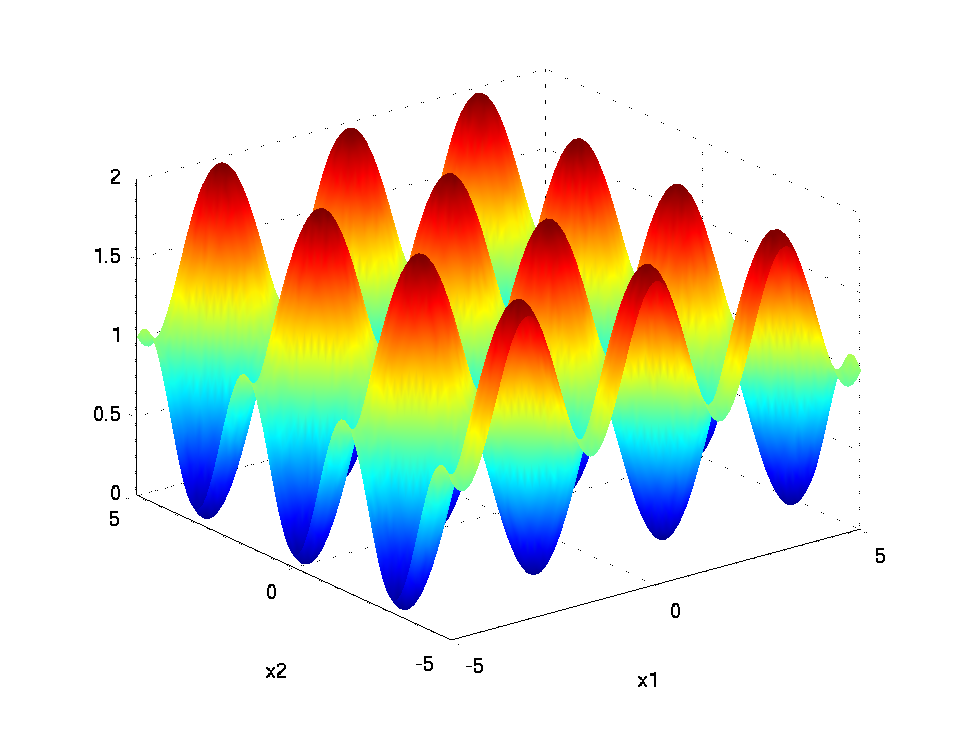
\includegraphics[width=0.7\columnwidth]{figs/global_opt2.eps}
\end{center}
Hér er erfiðara að koma auga á hámarkið, en við finnum það m.þ.a. leysa 
\[\nabla f(x_1,x_2)=\left(\frac{\partial f}{\partial x_1},\frac{\partial f}{\partial x_2}\right)=\vec{0}\]
þ.e.
\begin{eqnarray*}
\frac{\partial f}{\partial x_1}=&2\cos(x_1)\left(-\sin(x_1)\right)=0 &\Rightarrow x_1=k\frac{\pi}{2},\;k\in\mathbb{Z}\\
\frac{\partial f}{\partial x_2}=&2\sin(x_2)\cos(x_2)=0 &\Rightarrow x_2=k\frac{\pi}{2},\;k\in\mathbb{Z}
\end{eqnarray*}
Athugum að einnig þarf að gilda $-5\leq k\frac{\pi}{2}\leq 5$. Skoðum tilsvarandi gildi á $f(x_1,x_2)$.
\end{lausnSYND}

Víðvær bestun er erfið vegna þess að almennt er erfitt að finna allar núllstöðvar $\nabla f$. Einnig er til í dæminu að $\nabla f$ sé hreinlega óskilgreint (ódiffranleg bestun) sem flækir málið ennfrekar.

Nálgunaraðferðir eins og t.d. \emph{sub-tour reversal} finna iðulega staðbundin há-/lággildi.

\begin{center}
  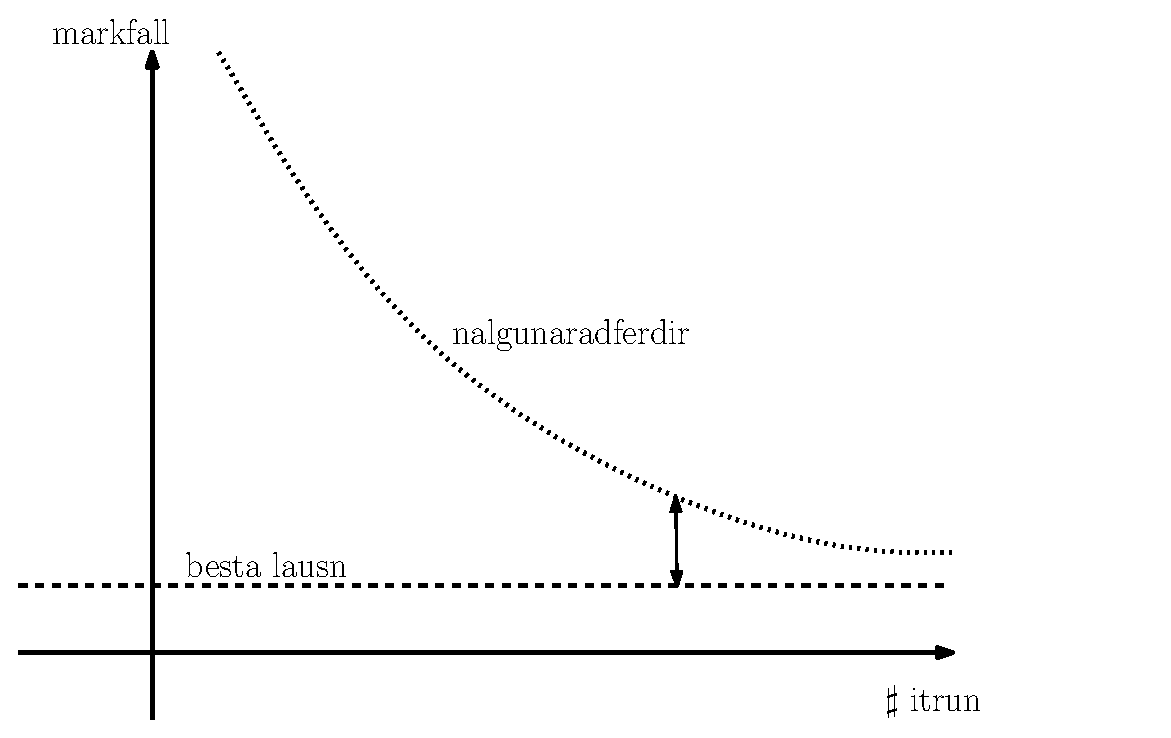
\includegraphics[width=0.5\columnwidth]{figs/global_approx.eps}
\end{center}

\section{Hermd kólnun}
\ath{Hermd kólnun} (e. simulated annealing) er algeng lausnaraðferð til að leysa víðværa bestun.
\begin{enumerate}
  \item Byrja með einhverja gjaldgenga lausn.
  \item Ítra:
  \begin{enumerate}
    \item Næsta lausn er valin af handahófi úr þeim lausnum sem eru \emph{nálægt} núverandi lausn. Hver þeirra verður fyrir valinu ræðst af líkindadreifingu sem ákvarðast af mismuni markfallsgilda ásamt \emph{hitastigi} ($T$) sem lækkar smám saman þegar ítrunum fjölgar.
    \item Af og til samþykkjum við lausnir sem eru \emph{verri} en sú besta sem fundist hefur fram að þessu. Tilgangur með því er að draga úr líkum á því að festa í staðbundnu lággildi.
    \subitem Þegar hitastigið ($T$) er hátt eru miklar líkur á að samþykkja verri lausn. Þegar það er lágt eru líkurnar litlar.
  \end{enumerate}
  \begin{aths}Analógía með kólnun á bráðnu gleri eða málmi:
  \begin{eqnarray*} \mbox{Bráðið kvartz}  & \begin{tabular}{cp{9cm}} 
    $\nearrow$ & Hröð kólnun: hrafntinna (óregluleg kristallsb.) \\
    $\searrow$ & Hæg kólnun: gler (regluleg kristallsbygging) \end{tabular}\\ &  \Rightarrow \mbox{lægri stöðuorka $\Rightarrow$ víðvært lágmark}\end{eqnarray*}
  \end{aths}
  Látum
  \begin{center}\begin{tabular}{lr}
    $z_c$ & markfall núverandi lausnar \\
    $z_n$ & markfall kandídats lausnar
  \end{tabular}\end{center}

  Samþykkjum kandídat ef $z_n\geq z_c$ (því hann er betri -- g.r.f. hámörkunarverkefni). Ef $z_n<z_c$ samþykkjum við kandídat með líkum
 \[ Pr\{\mbox{samþykkja}\}=e^{(z_n-z_c)/T} \]
\begin{aths}$\lim_{T\to0} e^{(z_n-z_c)/T}=0$ því $(z_n-z_c)<0$.\end{aths}
\end{enumerate}

\begin{samepage}
\subsection*{Dæmi um stöðvunarskilyrði}
\begin{enumerate}
  \item ákveðinn fjöldi ítrana hefur verið náð,
  \item hitastig náð einhverju tilteknu gildi,
  \item engin bæting á markfalli fundist í langan tíma.
\end{enumerate}
\end{samepage}

Þegar leit lýkur vitum við ekki hversu langt lausnin okkar er frá besta gildi (gætum jafnvel hafa slysast á þá bestu).

Sérsníða þarf reiknirit sem byggja á hermdri kólnun að sérhverri tegund verkefna. Það sama gildir um \ath{bannleit} (e. tabu-search 13.2 í H\&L) og \ath{erfðaalgrím} (e. genetic algorithms í 13.4 í H\&L).

\begin{lausn}[Nálgunarlausn á TSP \ref{daemi:tsp} fundið með hermdri kólnun]\hspace{.1cm}
  \begin{enumerate}
    \item Byrjum með einhverja sæmilega góða upphafslausn, t.d. $1\to2\to3\to4\to5\to6\to7\to1$, með $z_c=69$.
      \subitem Oft fæst þokkaleg upphafslausn með því að velja upphafspunkt af handahófi. Förum næst í þann punkt sem er í stystu fjarlægð frá upphafspunktinum og svo koll af kolli (gráðug aðferð).
    \item Notum \emph{sub-tour reversal} t.þ.a. finna lausnir í nágrenni núverandi lausnar.
      \subitem Veljum upphafs- og endapunkt af handahófi t.d. $1\to2\to3\to5\to4\to6\to7\to1$. Kandídatinn er gjaldgengur með $z_n=65$. 	\subsubitem Þar sem $z_n=65<69=z_c$ samþykkjum við $1\to2\to3\to5\to4\to6\to7\to1$ sem bestu lausn.
      \subsubitem Ef hins vegar $z_n>z_c$ þá er nýja lausnin verri. Samþykkjum hana með líkum $\exp\left\{\left(z_c-z_n\right)/T\right\}$.
    \item Hitastýring: Í upphafi má t.d. nota $T_1=0.2z_c$ og síðan $T_k=0.95T_{k-1}$, $k=2,3,4,...$
  \end{enumerate}

\end{lausn}
